
\documentclass[%
 aip,
 jmp,%
 amsmath,amssymb,
%preprint,%
 reprint,%
%author-year,%
%author-numerical,%
]{revtex4-1}

\usepackage{parskip,graphicx} 
\usepackage[utf8]{inputenc} %not clear effect
\usepackage[T1]{fontenc} %not clear effect
\usepackage[english]{babel}% not clear effect
\usepackage{float} %used for fixed tables with [H]
\usepackage{textcomp}
\usepackage{enumerate}
\usepackage{wrapfig}
\usepackage{amssymb}
\usepackage{epstopdf}
\usepackage{inputenc}
\usepackage{array}
\usepackage{booktabs}
\usepackage{subfig}
\usepackage[justification=centering]{caption}
\usepackage{array}% http://ctan.org/pkg/array	
\usepackage{float}
\usepackage[nottoc]{tocbibind}



\newcommand*{\citen}[1]{%
  \begingroup
    \romannumeral-`\x % remove space at the beginning of \setcitestyle
    \setcitestyle{numbers}%
    \cite{#1}%
  \endgroup   
}



\begin{document}


\title[A Simplified Derivation of the Hawking Effect and its Consequences]{General Relativity Presentation:\\ A Simplified Derivation of the Hawking Effect and its Consequences}% Force line breaks with \\


\author{Student: Daniel Prelipcean}
\affiliation{Jacobs University Bremen, 28759 Bremen, Germany%\\This line break forced with \textbackslash\textbackslash
}%

\date{December 10, 2016}% It is always \today, today,
             %  but any date may be explicitly specified

\begin{abstract}
The famous Hawking effect shows that a black hole radiates as if it were an ideal black body with temperature $T = \hbar c^3 / 8 \pi k_B G M$. Under reasonable assumptions, this can be seen as an implication of the Unruh effect, which is derived here using a simple, intuitive argument given for the case of a scalar field in one spatial dimension. Interesting consequences such as black hole evaporation and Hawking lifetime are further investigated giving numerical values as well. The final computation considers the observable universe as a black hole which evaporates in a bigger universe, thus enabling us to find the life span of our own universe.
\end{abstract}

\keywords{Unruh effect, Rindler coordinates, Planck radiation law, Hawking effect, black hole evaporation}
\maketitle


\section{Unruh Effect}

A phenomenon manifested even in flat spacetime is the Unruh effect. It states that an accelerating observer in Minkowski vaccum state will observe a thermal spectrum of particles.
\subsection{Rindler coordinates}
Uniform acceleration is defined as a constant acceleration $\alpha > 0$ in an instantaneous inertial frame attached to the observer O', such that O' is at rest in this frame (as depicted in fig. \ref{framespic}). The acceleration $dv/dt$ in the lab frame is related to $\alpha$ by the Lorentz transformation formula [\citen{lorentztransformations}]:
\begin{equation}
\frac{dv}{dt}= a = \gamma^{-3} \alpha
\end{equation}
where the Lorentz factor  $\gamma(t) = \left(1-v(t)^2/c^2\right)^{-1/2}$ is time dependent. 
\begin{figure}[H]
\centering
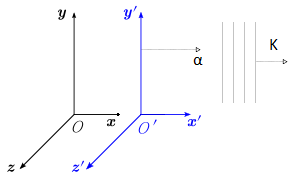
\includegraphics[width=1.0\linewidth]{frames.png}
  \captionof{figure}{Moving frame O' with constant proper acceleration $\alpha$ seen by the observer at rest in the reference frame O}
  \label{framespic}
\end{figure}
The proper and lab times are related by $d\tau=dt \gamma^{-1}$ and after all integration steps with $t(\tau=0)=0=v(\tau=0)$ to make the integration constants vanish, we obtain:
\begin{align}
    t(\tau) & =\dfrac{c}{\alpha}\sinh{\dfrac{\alpha \tau}{c}} \\
    v(\tau) & =c\tanh{\dfrac{\alpha \tau}{c}} 
    \label{vtau}\\
    x(\tau) & =\dfrac{c^2}{\alpha}\cosh{\dfrac{\alpha \tau}{c}} 
\end{align}
These coordinates satisfy the relation:
\begin{equation}
x^2=t^2+\alpha^2
\end{equation}
These describe the well known hyperbolic orbits (fig. \ref{rindlercoordinatespic}) of the accelerated Rindler [\citen{rindlercoordinates}] observer in $\hat{x}$ direction.  The hyperboloids are asymptoting the null paths $x= -t$ in the past and $x= t$ in the future. Note that the observer travels from past null infinity to future null infinity rather than timelike infinity as would be reached by geodesic observers.\\
\begin{figure}[H]
\centering
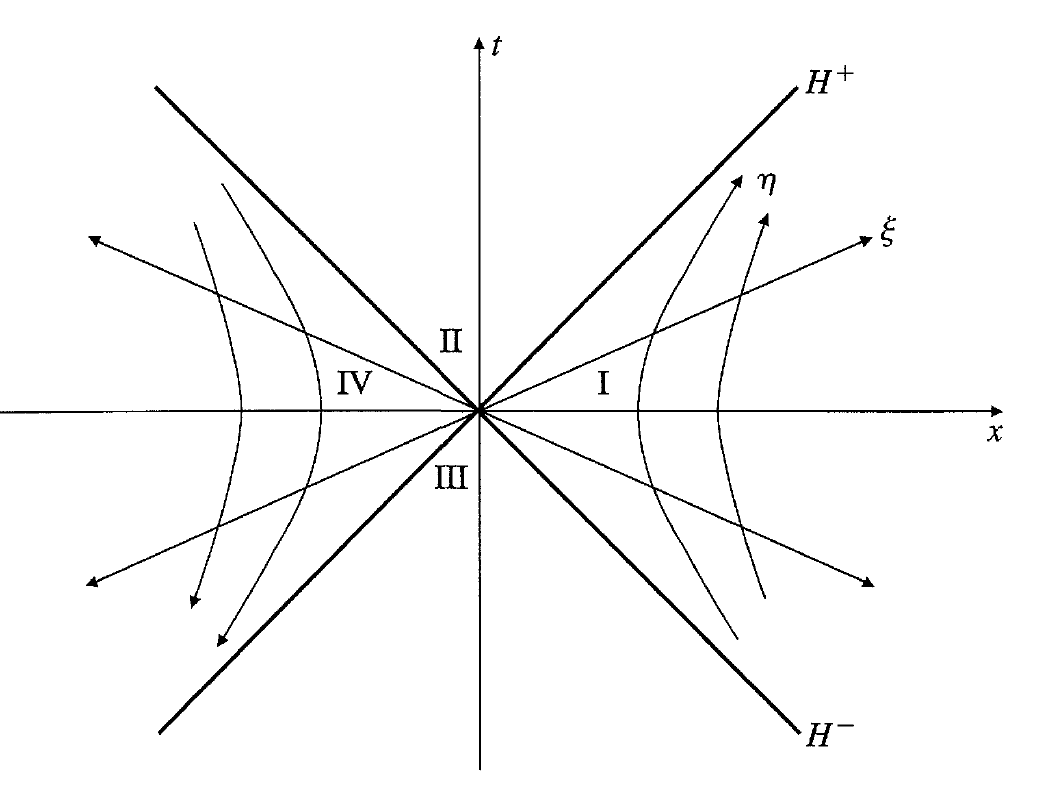
\includegraphics[width=1.0\linewidth]{rindlercoordinatespic.png}
  \captionof{figure}{Minkowski space time in Rindler coordinates. Region I is the region accessible to an observer undergoing a constant proper acceleration $\alpha$ in the $+\hat{x}$ direction. Similarly, new coordinates $t = \frac{1}{a} e^{a\xi} \sinh{a \eta}$ and  $x = \frac{1}{a} e^{a\xi} \cosh{a \eta}$ can be defined to have a better understanding of the Minkowski chart [\citen{carollspacetime}]}
  \label{rindlercoordinatespic}
\end{figure}

\subsection{Planar-wave field}

The derivation used in this subsection follows Paul M. Alsing and Peter W. Milonni in [\citen{simplifiedderivation}]. Consider now a plane-wave field of frequency $\nu_k$ and wave vector $\vec{K}$ with $\vert\vec{K}\vert = K = \nu_k/c$ parallel or anti-parallel to the direction x along which the observer is accelerated. Lorentz transformation formulae [\citen{lorentztransformations}] also give the instantaneous rest frame of the observer the frequency $\nu_k\prime$ of this field:
\begin{align}
    \nu_k\prime(\tau) & = \dfrac{\nu_k-Kv(\tau)}{\sqrt{1-v^2(\tau)/c^2}}
\end{align}
Plugging in the definition of $v(\tau)$ from equation (\ref{vtau}) gives:
\begin{equation}
    \nu_k\prime(\tau)= \dfrac{\nu_k \left[1- \tanh{\dfrac{\alpha \tau}{c}}\right]}{\sqrt{1-\tanh{\dfrac{\alpha \tau}{c}}^2}}=\nu_k \exp{\dfrac{-\alpha \tau }{c}}
\end{equation}
For $\alpha \tau /c \ll 1$ and by expanding the exponential function around 0 gives:
\begin{equation}
    \nu_k\prime=\nu_k \left( 1 \mp \dfrac{\alpha \tau}{c} \right)
\end{equation}
which is exactly a time dependent Doppler effect. Now we are interested in finding the phase of such a planar wave. This is time dependent as well:
\begin{equation}
    \phi(\tau)=\int \nu_k\prime(\tau) d\tau = - \nu_k \dfrac{c}{\alpha}\exp{-\dfrac{\alpha \tau }{c}}
\end{equation}
We can say for the energy frequency spectrum that:
\begin{equation}
    E(\nu) \propto \left| \int_{-\infty}^{+\infty} \exp{(i\omega_k\tau)} \exp{(i\phi)} d\tau \right|^2
\end{equation}
Plugging in our definitions for $\nu$ and $\phi$ gives:
\begin{equation}
    E(\nu) \propto \left| \int_{-\infty}^{+\infty} \exp{(i 2 \pi \nu_k\tau)} \exp{\left(-i \nu_k \dfrac{c}{\alpha}\exp{\left(-\dfrac{\alpha \tau }{c}\right)}\right)} d\tau \right|^2
\end{equation}
Evaluating this complicated integral yields in the end:
\begin{equation}
    E(\nu) \propto \left(\exp{\left(\dfrac{4 \pi^2\nu_k}{\alpha}\right) - 1 \right)}^{-1}
\end{equation}
From Planck`s radiation Law for a black body, we have:
\begin{equation}
    E(\nu) \propto \left(\exp{\left(\dfrac{h \nu}{k_B T}\right)}-1 \right)^{-1}
\end{equation}
By simply comparing the Planck factors from the exponential, we obtain the Unruh temperature:
\begin{equation}
    T_{Unruh} = \dfrac{\hbar \alpha}{2 \pi k_B c}
    \label{tunruh}
\end{equation}

\section{Hawking Effect}
In a very small region very close to the event horizon, the space-time is stretched so strongly that we can approximate it with a Minkowski flat space-time, in order to allow us to use the Unruh effect reasoning (for more details see ref. [\citen{carollspacetime}]). The acceleration of a particle is then replaced by the surface gravity [\citen{surfacegravity}] of a black hole:
\begin{equation}
    \alpha \rightarrow \kappa = \dfrac{c^4}{4MG}
\end{equation}
\begin{figure}[H]
\centering
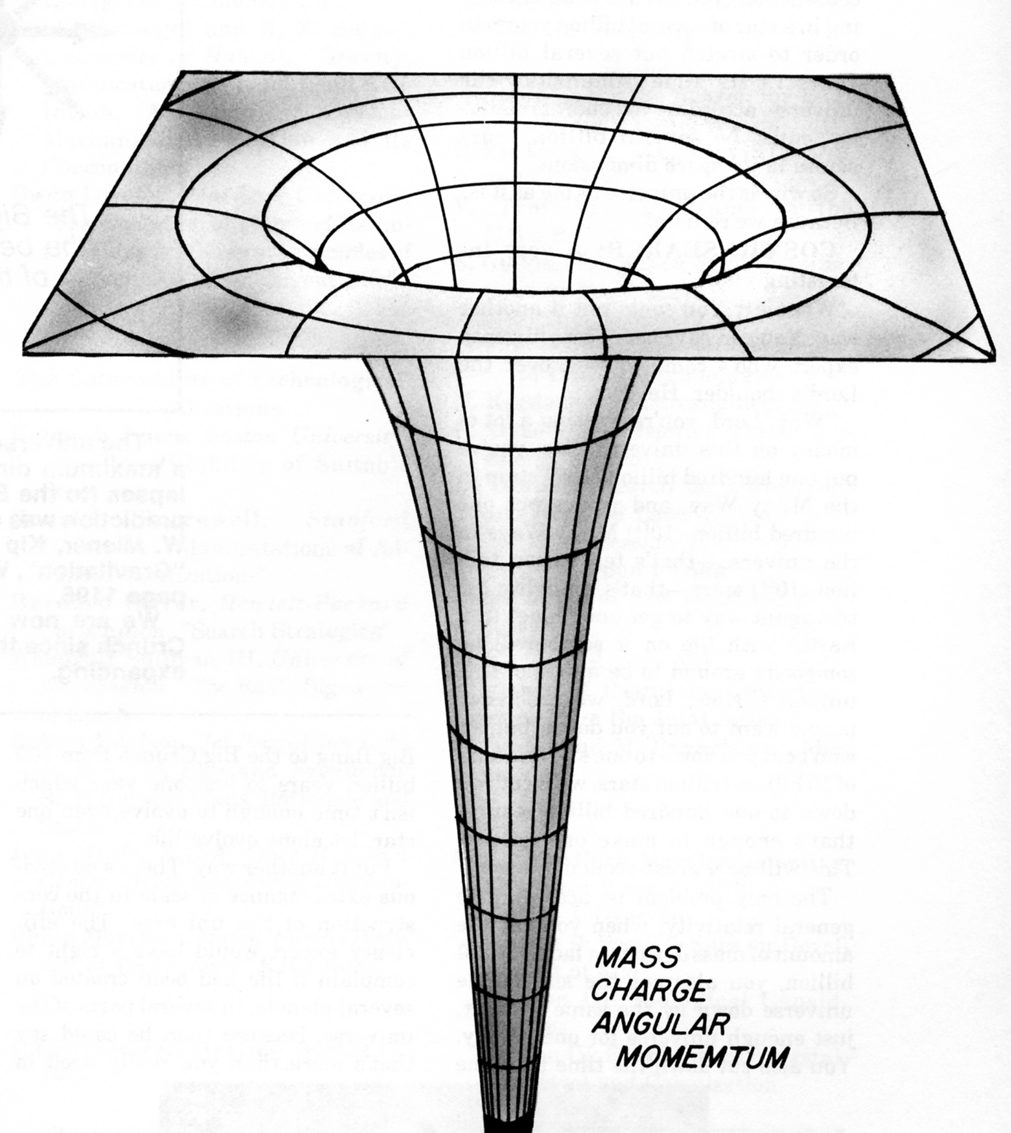
\includegraphics[width=1.0\linewidth]{bhspacetime.png}
  \captionof{figure}{Representation of a black hole suggesting how space-time is curved [\citen{bhspacetime}]}
  \label{bhspacetimepic}
\end{figure}
Plugging this into equation (\ref{tunruh}) yields the Hawking Temperature of a black hole seen as a radiating black body:
\begin{equation}
    T_{HW} = \dfrac{\hbar c^4}{8 \pi k_B G M} \sim \dfrac{1}{M}
\end{equation}
This result implies that the more massive a black hole is, the lower its temperature and implicitly its emitted radiation. In fact, most of the black holes have a temperature lower than the Cosmic Microwave Background $T_{CMB} = 2.73$ K. For a black hole to be in "thermal equilibrium" with the background, it should have a mass of $M\approx 1.5 \cdot 10^{19}$ kg. An object with such a mass is the asteroid 140 Siwa [\citen{asteroid}] orbiting in the asteroid belt.

\section{Quantum fluctuations}
A plausibility argument [\citen{schutz}] follows from Heisenberg`s uncertainty relation $\Delta E \cdot \Delta t \ge \hbar/2$. According to quantum field theory, ordinary space is filled with "vacuum fluctuations" in electromagnetic fields,  which consist of pairs of photons being produced at one event and recombining at another. Such pairs violate conservation of energy, but if they last less than the Heisenberg time, they violate no physical law.\\

As we suggested before, space-time near the horizon of the black hole can be considered flat, where fluctuations are happening. These particles are then emitted giving the Hawking effect.
\begin{figure}[H]
\centering
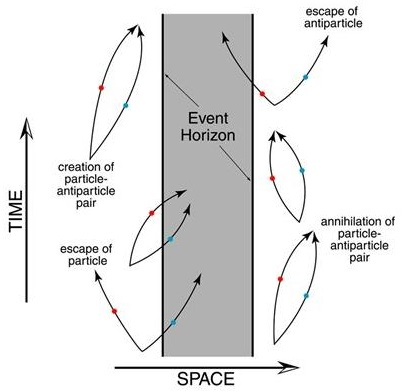
\includegraphics[width=1.0\linewidth]{HawkingRadiation1.jpg}
  \captionof{figure}{Vacuum fluctuations may result in one of the particle/antiparticle pair crossing the event horizon, remaining trapped inside the black hole, and the other escaping to infinity as Hawking radiation [\citen{hawkradpicture}]}
  \label{bhspacetimepic}
\end{figure}

\section{Evaporation of Black Holes}
For an observer at infinity, the black hole radiates particles via Hawking effect. Since these particles have energy, it seems that energy has been extracted from the black hole, which will reduce its mass. We are now interested in finding the rate of this energy release, i.e. the black hole evaporation. A very intuitive dimensional analysis argument (see ref. [\citen{hartlegrav}]) is used to guess the steady rate $dM/dt$ at which the black hole loses mass by Hawking radiation as determined by a stationary observer at infinity whose proper time is $t$.\\

\newpage

Since it is a quantum mechanical process, it is expected to be proportional to Planck`s constant $\hbar$ $(1J= kg m^2 s^{-2})$. Then we need a combination which yields the proper units:
\begin{equation}
    \left( \dfrac{dM}{\hbar dt}=\right) \dfrac{kg}{J s}= \dfrac{kg}{\dfrac{kg m^2}{s^2}s}=\dfrac{1}{m^2}
\end{equation}
Such a reasonable (and in fact  unique) combination is:
\begin{equation}
    \left( \dfrac{c^4}{(G M)^2} = \right) \dfrac{\left(\dfrac{m}{s}\right)^4}{\left( \dfrac{m^3}{kg s^2} kg\right)^2} = \dfrac{1}{m^2}
\end{equation}
Therefore, we obtain the evaporation rate as seen by a distant observer to be:
\begin{equation}
    \dfrac{dM}{dt} = \dfrac{- \nu c^4 \hbar}{(GM)^2}
\end{equation}
where the minus sign denotes the mass reduction over time and $\nu = 1/(15.360 \pi)$ is a positive dimensionless constant. This value for $\nu$ neglects the effect of geometry on the radiation as it propagates, which slightly alters the correct value. By integrating, one obtains for a black hole with life time $t_0$:
\begin{equation}
    M(t) = \left[ 3 \hbar \nu (t_0 - t)\right]^{1/3}
    \label{mt}
\end{equation}
\begin{figure}[H]
\centering
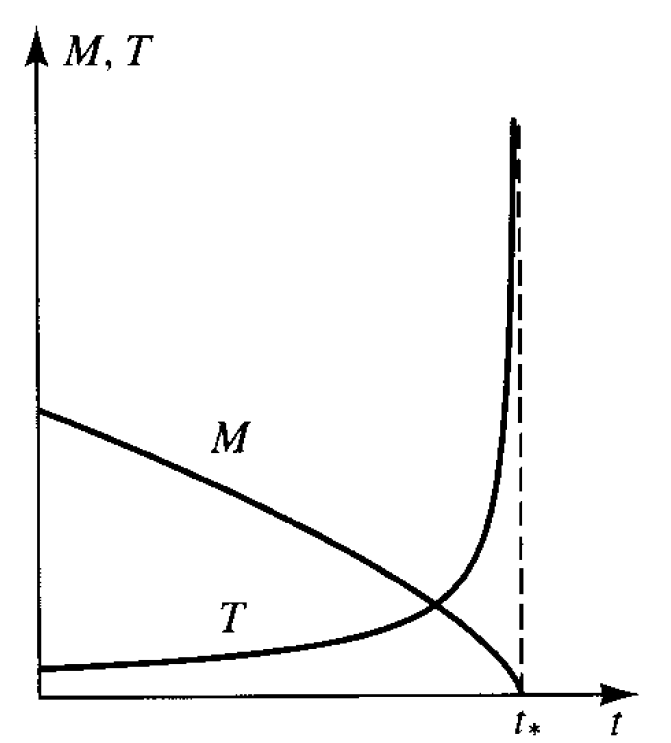
\includegraphics[width=1.0\linewidth]{masstemptime.png}
  \captionof{figure}{As the mass decreases, the temperature rises. The black hole therefore radiates at increasingly rapid rates as it shrinks, resulting in an explosive end [\citen{hartlegrav}]}
  \label{bhspacetimepic}
\end{figure}

\newpage

By turning around equation (\ref{mt}), one obtains an estimate for the finite life time of a spherical black hole which completely evaporates due to Hawking Radiation:
\begin{equation}
    \tau_{Hw} \approx \dfrac{1}{3\nu }\dfrac{M^3}{\hbar} = 8.3 \cdot 10^{-26} \left( \dfrac{M}{1 g} \right)^3 s \sim M^3
    \label{evaptime}
\end{equation}
This implies that almost all black holes have a greater life time than the current 14-billion-years age of the universe, but some black holes of $10^{14}$ g would end their lifetime in the present. It is possible for such a small black hole to form in the very early universe. For a brief second before its explosion, it would have a luminosity about 0.1$\%$ of the Sun’s luminosity, but in spectrum it would be very different, emitting primarily in $\gamma$-rays. A primordial black-hole evaporation would probably be visible only if it happened in our own Galaxy. No such events have been identified. 


\begin{figure}[H]
\centering
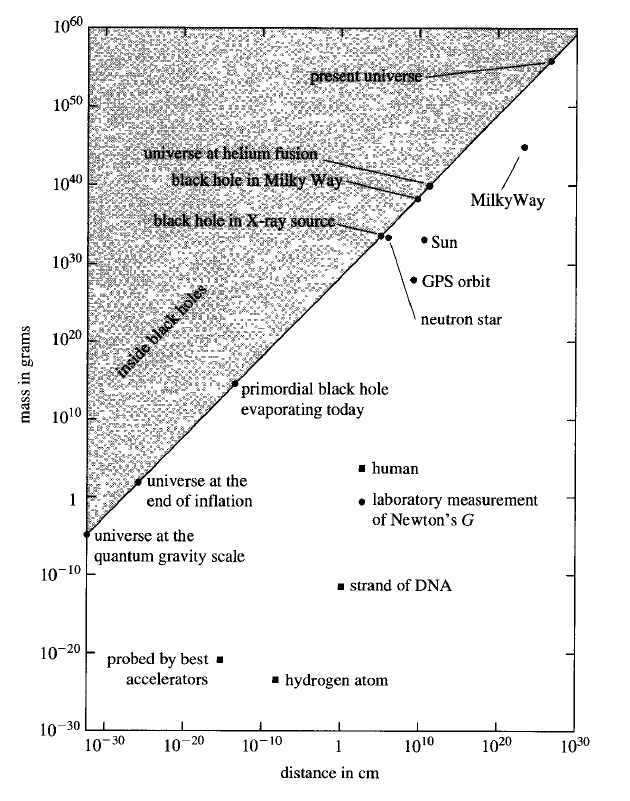
\includegraphics[width=1.0\linewidth]{massdistribution.png}
  \captionof{figure}{The characteristic mass M vs. characteristic distance R for phenomena for which gravity is important. Those above the diagonal line are unobservable, as they take place inside a black hole [\citen{hartlegrav}]}
  \label{massdistrib}
\end{figure}
\hfill
\newpage


\section{Lifetime of the observable universe}

As a final exercise, an interesting and fun computation is carried out. As seen in fig. \ref{massdistrib}, the universe can be considered as black hole. Then it radiates in a "bigger" universe, and we could compute the lifetime of our universe as seen by an observer outside. Different approximations for the mass of the universe are used. Consider the mass of the universe made out of ordinary matter to be $M_1 = 10^{56}$ g [\citen{massuniverse}]. Plugging this into equation (\ref{evaptime}) gives $t_1 = 8.3 \cdot 10^{142} s = 2.63 \cdot 10^{135}$ years. However, this mass would not reach the density needed for black hole.If now we take into account, besides ordinary matter ($\approx 4.9 \%$ of the universe), the dark matter ($\approx 26.8 \%$ of the universe) as well, then we obtain even a longer lifetime. Since dark energy, by convention, does not count as "matter", then the mass of the universe is $ M_2 = \dfrac{4.9 + 26.8}{4.9} \cdot 10^{56} g = 6.46 10^{56} g$. This gives $t_2 = 2.24 \cdot 10^{145} s = 7.09 \cdot 10^{137}$ years. A different approach is to consider the average density (light and dark matter) and the volume of the observable universe. The mass is then $M_3 = \rho \cdot V = 3 \cdot 10^{-30} \dfrac{g}{cm^3} \cdot 14 \cdot 10^9$ ly  $= 3 \cdot 10^{55} g$ [\citen{massuniverse3}]. This gives a time of $t_3 = 2.241 \cdot 10^{141} s = 7.1 \cdot 10^{133}$ years.


\bibliography{bibliography.bib} 

\end{document}
